\documentclass[a4paper,11pt,openright,openbib]{report}
\usepackage[portuges]{babel}
\usepackage[T1]{fontenc}
\usepackage{ae}
\usepackage[utf8x]{inputenc}
\usepackage[pdftex]{graphicx}
\usepackage{url}
\usepackage{listings}
\usepackage{verbatim}
\usepackage{acronym}
\usepackage{multirow}
\usepackage[section,above,below]{placeins}
\usepackage{enumerate}

\usepackage[a4paper, pdftex, bookmarks, colorlinks, linkcolor=black, urlcolor=blue]{hyperref} %por linkcolor=cor para ter os links com cor.
\usepackage[a4paper,left=2.5cm,right=2.5cm,top=3.5cm,bottom=3.5cm]{geometry}
\usepackage{colortbl}
\usepackage[margin=10pt,font=small,labelfont=bf]{caption}
\usepackage{mdwlist}
\usepackage{tocbibind}

%definições

\setlength{\parindent}{0cm}
\setlength{\parskip}{2pt}

%def codigo inlining (trocar xml (nome de ambiente) e XML por linguagem correcta (ex. JAVA, C, etc)
\lstnewenvironment{xml}{\lstset{
	language=XML,
	basicstyle=\small,
	extendedchars=false,
	inputencoding=utf8x,
	breaklines=true,
	showstringspaces=false,
	keywordstyle=\scriptsize\bfseries,
	basicstyle=\scriptsize\sf,
	breakautoindent=false}
}{}


% Title Page

\title{
	\begin{tabular}{l r}
	\large{Universidade do Minho} & \multirow{3}{*}{
\includegraphics[width=0.2\textwidth]{imagens/UM}} \\
	\large{Licenciatura em Engenharia Informática} & \\
	\large{Processamento de Linguagens} & \\
	\\
	\\
	\Large{\textbf{Processamento da Wikipedia}} & \\
	\large{Ano Lectivo de 2010/2011} & \\
	\\
	\\
	\\
	\end{tabular}
}


\author{
	\begin{tabular}[t]{l}
	\\
	\\
	54745 \textbf{André Pimenta} \\
	54738 \textbf{João Gomes} \\ 
	54802 \textbf{Milton Nunes} \\
	\\ 
	\end{tabular}
}

\date{\today}


\begin{document}


\maketitle
\pagenumbering{roman}


%resumo
\begin{abstract}
Este projecto consiste sobretudo na utilização de expressões regulares. Pretende-se, através do uso do Special Export, que sejam exportadas páginas do wikipedia para que depois através da identificação de determinados padrões em XML, se possam definir expressões regulares que extraiam os dados que pretendemos, isto com o auxilio das ferramentas Flex.\\
Através da linguagem C são tratados os dados e criado um output, em HTML, com os resultados obtidos.\\
Neste relatório daremos sobretudo importância aos padrões de XML encontrados, às expressões regulares que desenvolvemos e também ao output do trabalho, ou seja ao nosso produto final, para além de um diagrama de estados referente a todas as expressões importantes.\\

\end{abstract}


%\chapter*{Agradecimentos}
%\addcontentsline{toc}{chapter}{Agradecimentos}

%conteudo
\tableofcontents
%\listoffigures
%\listoftables

%documento


%\clearpage

\pagestyle{headings}
\pagenumbering{arabic}
\newpage
\chapter{Contextualização}

\section{Estrutura}
O presente relatório é constituído por 3 capítulos: \textbf{Contextualização} onde é feita uma breve contextualização do problema dentro da engenharia de processamento de linguagens,\textbf{Desenvolvimento do processador da Wikipedia} onde são descritos todos os passasos do desenvolvimento do processador do wikipedia e \textbf{Conclusão} onde é feita uma breve conclusão sobre o trabalho realizado.

\section{Motivação e objectivos}
O desenvolvimento deste trabalho implica o uso de expressões regulares e o uso da ferramenta Flex. As expressões regulares, como foi leccionado nas aulas de Processamento de Linguagens, permite-nos identificar sequências, palavras ou padrões de caracteres em ficheiros.\\
Isto torna-se muito útil pois permite-nos retirar de um ficheiro determinados padrões para usar-mos posteriormente no nosso software, que é o que se pretende neste trabalho, uma selecção de determinados padores para depois usar como output.\\
Para isso usa-se também o Flex, que consiste numa ferramenta que vai identificar no ficheiro XML os padrões definidos por nós através de regras definidas através de expressões regulares.\\
É portanto, nosso objectivo aplicar as expressões regulares e o uso da ferramenta Flex, desenvolvendo as suas potencialidades e adquirindo o máximo de conhecimento acerca destas.\\
\section{Introdução}
Pretende-se com este trabalho a aplicação dos conhecimentos adquiridos nas primeiras aulas da disciplina de Processamento de Linguagens.
O trabalho consiste em criar um filtro, através da aplicação de expressões regulares, para estruturar um conjunto de dados extraidos de páginas da Wikipedia, em formato XML.\\
O output deste filtro,que foi obtido através do Flex, será gerado em páginas HTML contendo as informações extraídas, depois de estas serem tratadas através de algumas funções desenvolvidas na linguagem C.\\

\newpage
\chapter{Desenvolvimento do processador da Wikipedia}
\section{Expressões Regulares}
Para criar as expressões regulares é importante que antes sejam identificados os padrões em XML que representem os conteúdos que se pretendem retirar do texto a processar.\\
Portanto foi preciso analisar os ficheiros em XML extraídos do Wikipedia e concluimos que os seguintes padrões definem os conteúdos que pretendemos:\\
\begin{figure}[!htb]
     \centering
     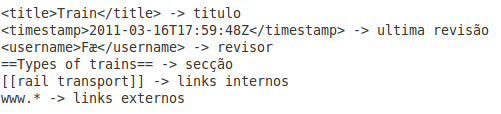
\includegraphics[scale=0.8]{imagens/er2.png}
	\label{Padrões das expressões}
\end{figure}  
	\\  
	
De referir que por links externos consideramos todos os links iniciados por 'www.' e represente dominios validos, e não apenas os que se encontram na secção de links externos das respectivas paginas do wikipedia.\\
Nas secções consideramos também apenas as secções e não as subsecções.\\


Encontrados os padrões que indicam os conteúdos definidos no enunciado do trabalho desenvolvemos as expressões regulares, e através do usod do egrep cofirmamos se os resultados eram os pertendidos.\\

\begin{figure}[!htb]
    \centering
    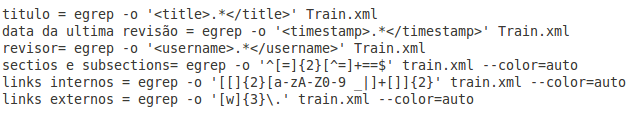
\includegraphics[scale=0.8]{imagens/er1.png}
\end{figure}  

\section{Expressões Regulares e estados correspondentes}
Com as expressões apresentadas acima conseguimos filtrar toda as informação que pretendemos, no entanto esta ainda tem de ser tratada e em alguns casos ( como o da revisão ) para facilitar e melhorar o uso destas mesmas expressões usamos estados no flex.\\
Definimos então os seguintes estados:
\begin{itemize}
	\item page - sempre que que é encontrada a etiqueta <page> entramos dentro do estado page onde se poderá encontrar toda a informação que pretendemos obter das respectivas paginas do Wikipedia.
	\begin{figure}[!htb]
		\centering
		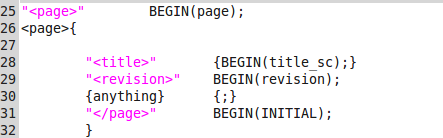
\includegraphics[scale=0.5]{imagens/page.png}
	\end{figure}  
	\item title - sempre que que é encontrada a etiqueta <title> e nos encontramos dentro do estado page entramos dentro do estado title onde se encontra o titulo da pagina wikipedia a ser processado.\\
	\begin{figure}[!htb]
		\centering
		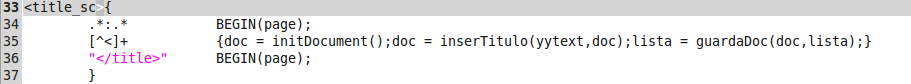
\includegraphics[scale=0.5]{imagens/title.png}
	\end{figure}
	\item revisão - sempre que é encontrada a etiqueta <revison> passaremos então para o estado revisão onde se encontra a informação relativa á revisão de documento e onde poderemos passar para o estado autor ou estado data de revsão.\\
	Dentro deste quando se encontrar a etiqueta </revision> abandonará-se este estado e passa-se para o estado que precede este, o estado page.\\
	\begin{figure}[!htb]
		\centering
		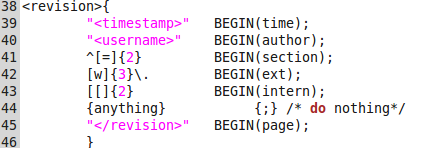
\includegraphics[scale=0.5]{imagens/revision.png}
	\end{figure}
	\item autor - este estado pode ser encontrado sempre que se encontrar a equita <username> dentro do estado revisao.\\
	Dentro deste estado encontrase o nome do autor da ultima revisão até se encontrar a etiqueta </author> que faz com que passemos ao estado anterior revisão.\\
		\begin{figure}[!htb]
		\centering
		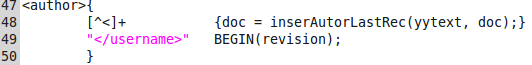
\includegraphics[scale=0.5]{imagens/author.png}
	\end{figure}
	
	\item data de revisão - entramos neste estado sempre que encontramos a etiqueta <timestamp> e estamos dentro do estado revision, dentro deste estado temos acesso á data da ultima revisão feita no documento.\\
	Este estado é abandonado quando se encontra a etiqueta </timestamp> e passamos para o estado anterior.\\
	\begin{figure}[!htb]
		\centering
		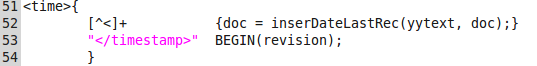
\includegraphics[scale=0.5]{imagens/time.png}
	\end{figure}
	\item ligação interna - estando dentro do estado revison sempre que se encontra a expressão "[[" o estado de ligação interna é activado.\\ Dentro deste encontra-se uma ligação interna até voltar a encontrar "]]" ou ' | ' ( este é encontrado sempre que exitem ligações internas com o mesmo nome mas que podem ser identificadas com nomes diferntes.)\\
	\begin{figure}[!htb]
		\centering
		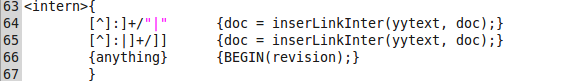
\includegraphics[scale=0.5]{imagens/intern.png}
	\end{figure}
	\item ligação externa - as ligações externas encontram-se sempre que se encontra a expressão "www.", após encontrar-mos este padrão entramos dentro do estado ligação externa. Dentro do estado de ligação externa podemos encontrar todas as referencias a ligações externas da pagina Wikipedia.\\
	\begin{figure}[!htb]
		\centering
		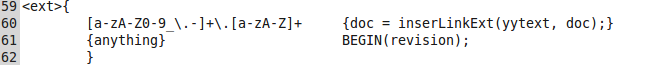
\includegraphics[scale=0.5]{imagens/ext.png}
	\end{figure} 
	\item secção - sempre que se encontrar a expressão "==" entraremos no estado de secção dentro desta encontram-se todas as secçõas da pagina Wikipedia até se encontrar a expressão "==" que faz com que voltemos ao estado revision.\\
	Devemos dar atenção neste estado que podemos estar perante subsections que são identificados com a expressõa "===".\\
		\begin{figure}[!htb]
		\centering
		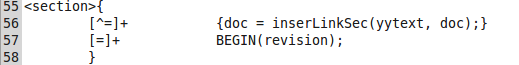
\includegraphics[scale=0.5]{imagens/section.png}
	\end{figure} 
\end{itemize}
\newpage
\section{Estrutura de Dados}
Depois de definidas as expressões regulares e utilizando o Flex foram extraídos os conteúdos pretendidos. Para que esses dados pudessem ser tratados foi necessário criar uma estrutura de dados onde eles são guardados.
Definimos então a seguinte estrutura de dados:
\\
\\typedef struct links\{ \\
    char* nomeLinks;\\
	struct links *next;\\
\} *Links;
\\
\\
typedef struct Document\{ \\
	char* titulo;\\
	char* autorLastRev;\\
	char* dateLastRev;\\
	int nInter;\\
	Links linkInter;\\
	int nExt;\\
	Links linkExt;\\
	int nSec;\\
	Links linkSec;\\
\} *Docs, DOC;
\\
\\
typedef struct listDocs\{ \\
	Docs doc;\\
	struct listDocs *next;\\
\} *List;
 \\
 
Esta estrutura permite-nos guardar os dados extraidos, isto é, permite nos guardar o titulo, o autor, a data da última revisão, o número de links externos/internos e quais são, e o número de secções e os seus nomes para cada pagina da Wikipedia contida no ficheiro XML.\\
Desta forma conseguimos tratar os dados(e.g ordenar todo alfabeticamente) para que depois conseguissemos gerar o output como pretendemos.\\
\section{Makefile}

Apresentamos a Makefile que por nós desenvolvida e que vêm permitir a instalação do programa de uma forma simples e correcta.\\
A criação desta Makefile é importante pois vêm juntar varios comandos que seriam necessários executar para que se corresse o programa. Desta forma com o simples comando make install temos o programa pronto a executar.\\ 


\begin{figure}[!htb]
     \centering
     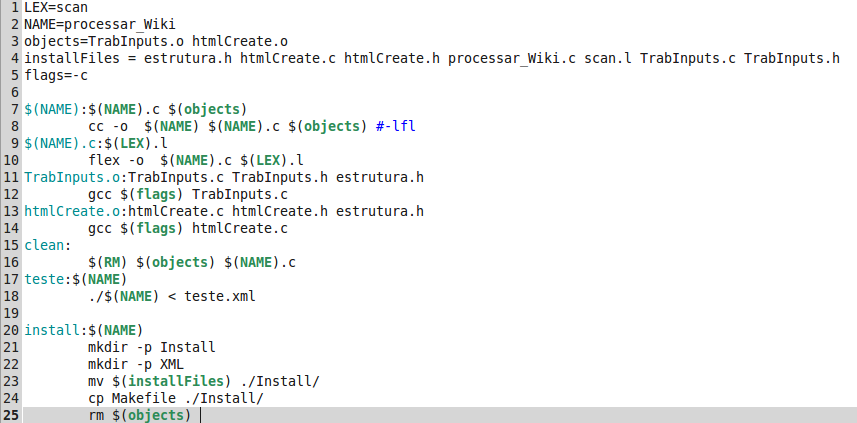
\includegraphics[scale=0.42]{imagens/makefile.png}
	\caption{Makefile}
\end{figure}  
%\newpage
\section{Diagrama de Estados}
Desenvolvemos também o nosso diagrama de estados, como ilustra a imagem abaixo. Esta representa os estados possíveis e o que leva a uma alteração dos mesmos.\\



\begin{figure}[!htb]
    \centering
    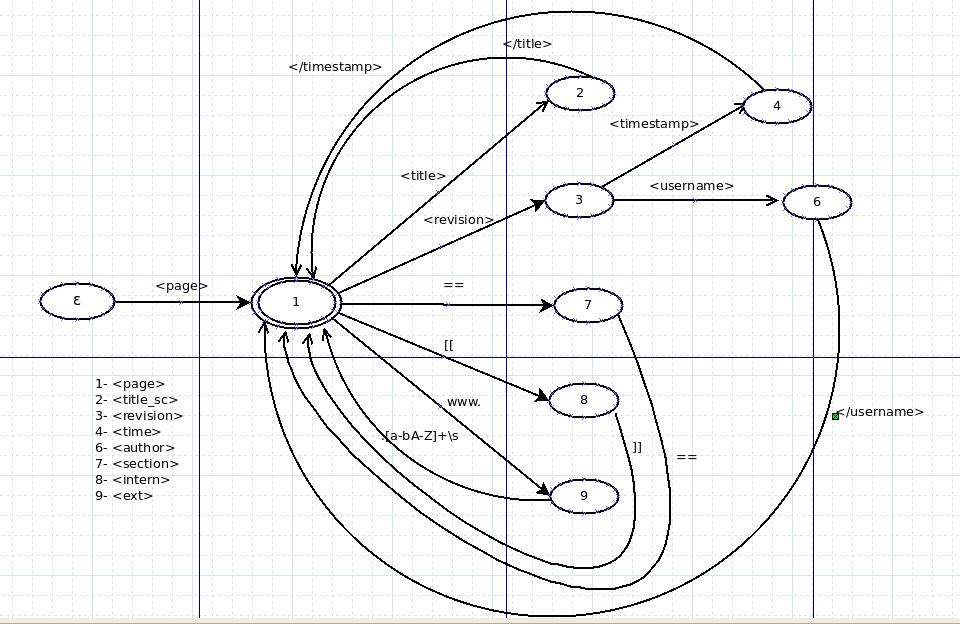
\includegraphics[scale=0.5]{imagens/diagrama.png}
	\caption{Diagrama de Estados}
\end{figure}  


No nosso diagrama de estados cada nodo identifica o estado em que se encontra. E cada aresta contém a expressão regular que leva à transição de estado para estado.


\newpage
\section{Testes estatísticos}

Concluida a aplicação decidimos realizar testes estatísticos. Estes testes pretendem verificar o tempo que demora a executar ficheiros de tamanhos diferentes.\\
Realizados os testes, aqui estão os resultados obtidos(pela seguinte ordem: Tamanho(MB), Tempo real(s) e Nº titulos do ficheiro):
\\
\\
2,4mb ---          0,4 seg   ---          100 artigos\\
9,5 mb      ---     0,8  seg       ---    500 artigos\\
17,5 mb       ---    1,1  seg   ---        1000 artigos\\
51,3 mb       ---      1,5  seg      ---   5000 artigos\\
90,8 mb       ---        2,3 seg  ---     10000 artigos\\
313,4 mb       ---        3,1 seg    ---  50000 artigos\\

Estes ficheiros foram criados através do ficheiro orgiginal da Wikipedia em português de serca de 3.6Gb usando a ferramenta felx para criar ficheiros com a quantidade de artigos que desejamos.\\


\begin{figure}[!htb]
    \centering
    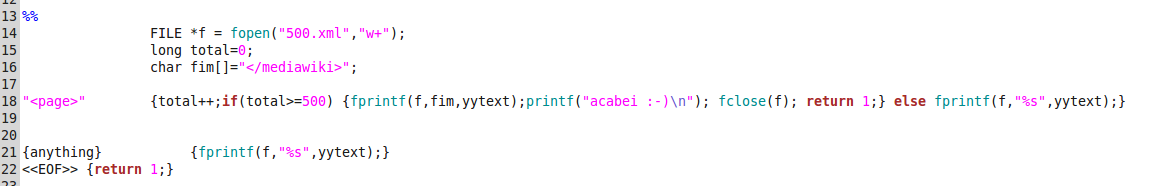
\includegraphics[scale=0.4]{imagens/files.png}
   \caption{Flex para cração de ficheiros}
\end{figure}

\newpage
\section{Output do programa}

Concluida a parte referente às expressões regulares e ao Flex, ou seja, assegurados os dados pretendidos no enunciado, a informação foi tratada, através de funções desenvolvidas na linguagem C, para posteriormente surgir no output do programa.\\
Esse output, tal como pedido no projecto, foi desenvolvido em HTML, e para cada ficheiro da wikipedia processedo é gerado um indice que contêm todas as paginas existentes no ficheiro XML a processar. Através deste indice podes aceder a todas as paginas e consultar os dados destas.\\
Apresentamos em baixo imagens que ilustram o outPut gerado pelo nosso programa.\\

\begin{figure}[!htb]
     \centering
     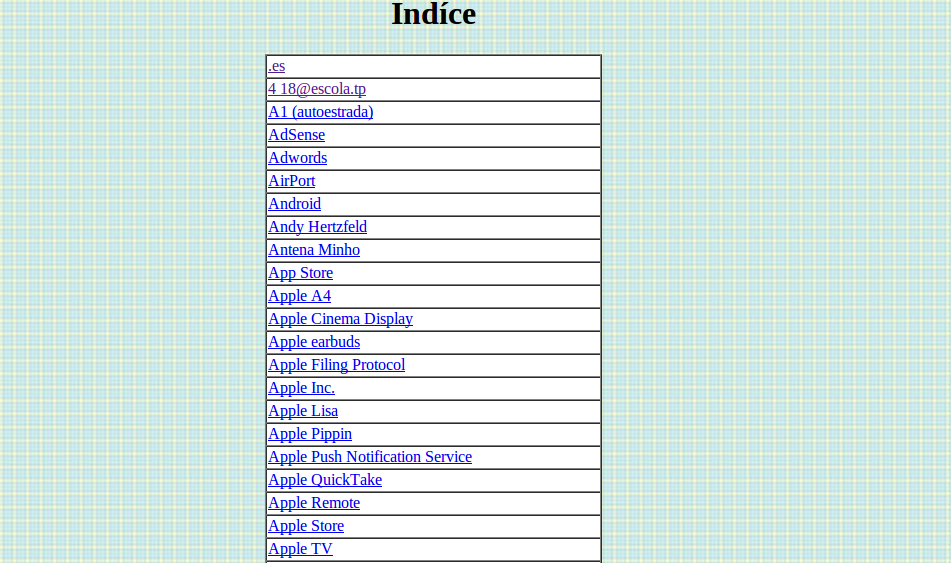
\includegraphics[scale=0.5]{imagens/indice.png}
     \caption{Indice}
\end{figure}  
\clearpage
\begin{figure}[!htb]
     \centering
     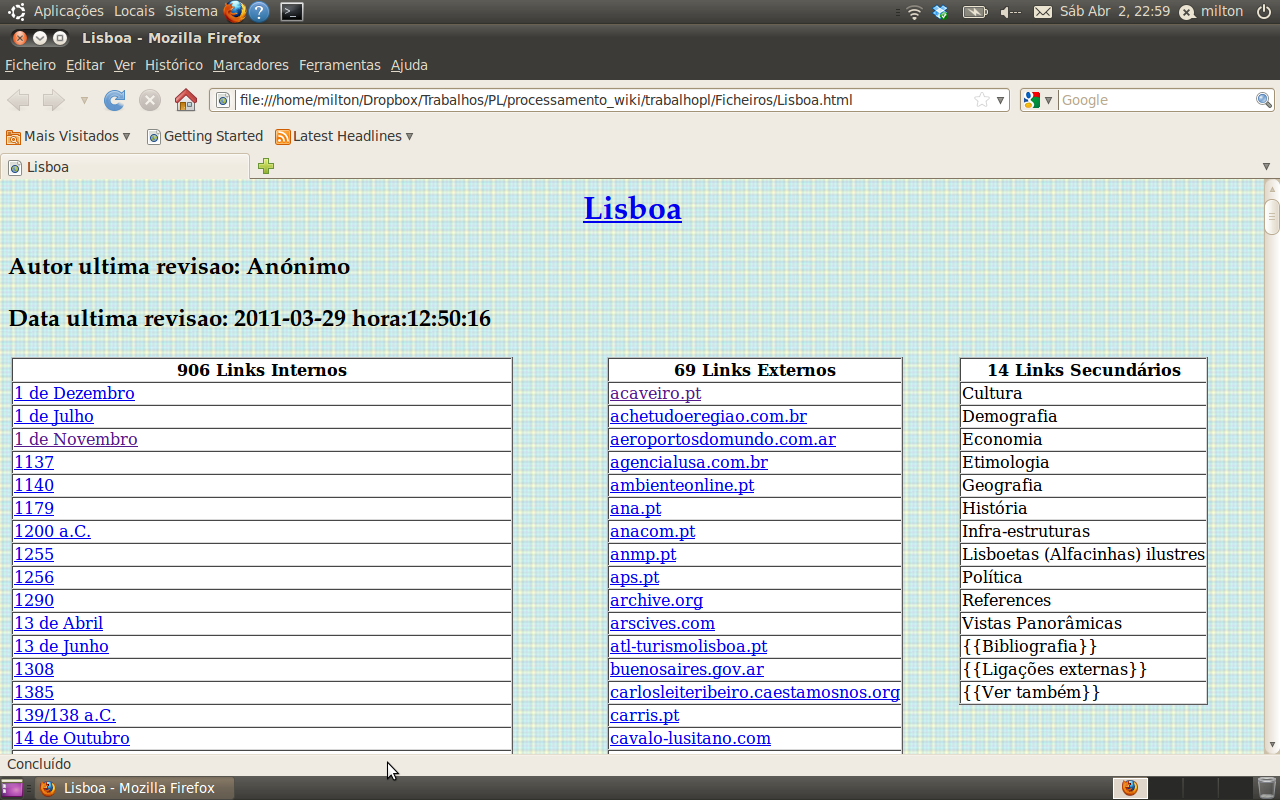
\includegraphics[scale=0.35]{imagens/print.png}
     \caption{Output do ficheiro lisboa.xml}
\end{figure}  


Para gerar este output é necessário correr o programa, utilizando os seguintes comandos: make install e ./processar\_Wiki nome\_ficheiro.xml \\
O output inclui todos os dados que o enunciado pretendia que retirássemos dos ficheiros XML, isto é, o título, autor da última revisão, data da última revisão, links externos, internos e secções. Estas últimas 3 encontram-se nas tabelas, como ilustra a imagem acima.



\chapter{Conclusão}

Este trabalho, apesar de ser um exemplo simples, ajudou-nos a perceber a potencialidade que as expressões regulares têm, isto é, o que nos permite fazer de forma simplificada.\\
As espressões regulares, revelam-se portanto, extremamente úteis para encontrar informação em ficheiros. Sendo que podemos estar a falar de milhares de ficheiros, com milhares de caracteres cada um, facilmente se percebe que a utilidade que oferece o uso das expressões regulares.\\

\label{c:conclusao}

\clearpage
\section{Elementos do Grupo}

\begin{figure}[!htb]
     \centering
     
\includegraphics[scale=0.13]{imagens/apr.jpg}
     \caption{André Pimenta}
     \label{André Pimenta}
\end{figure}
\begin{figure}[!htb]
     \centering
     
\includegraphics[scale=0.6]{imagens/jmbg.png}
     \caption{João Miguel}
     \label{João Miguel}
\end{figure}
\begin{figure}[!htb]
     \centering
     
\includegraphics[scale=0.1]{imagens/mfn.jpg}
     \caption{Milton Nunes}
     \label{Milton Nunes}
\end{figure}

\end{document}
